\section{Data Access}
\label{sec:databases}

%%%%%%%---- BEGIN ----  ----%%%%%%
\begin{frame}
  \frametitle{Databases and Data Aggregators}

  \begin{columns}[T]

      \begin{column}{.3\textwidth}
        \vspace{0.5em}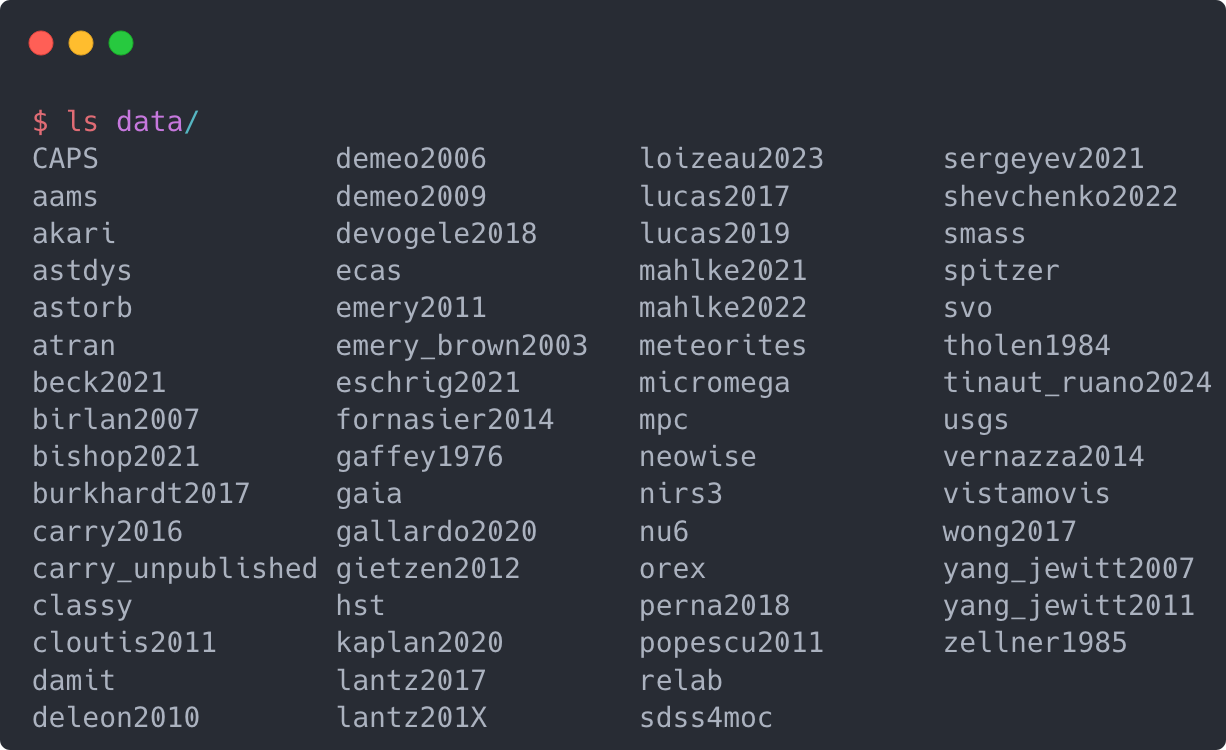
\includegraphics[width=.8\textwidth]{data_dir}\\
        \vspace{0.5em}
\includegraphics[width=.8\textwidth]{logo_astorb}\\
        \vspace{0.5em}
\includegraphics[width=.8\textwidth]{logo_mp3c}\\
        \vspace{0.5em}
\includegraphics[width=.8\textwidth]{logo_ssodnet}\\
      \end{column}


    \begin{column}{.7\textwidth}
      \begin{overlayarea}{\textwidth}{\textheight}
        \begin{onlyenv}<1>

          \vspace{1em}
          We all need data, we all generate data.\\
          \vspace{1em}
          \begin{itemize}[<.->]
            \item \emph{\bf Databases}
              \begin{itemize}[<.->]
                \item[$\circ$] Websites, CDS, on-request
                \item[$\circ$] Mostly static, single bibliographic reference
                \item[$\circ$] Mixture of formats
              \end{itemize}

            \vspace{0.5em}
            \item \emph{\bf Data Aggregators}
              \begin{itemize}[<.->]
                \item[$\circ$] Collection of data \emph{with processing}
                \item[$\circ$] Dynamic, large number of bibliography references
                \item[$\circ$] Uniform output
              \end{itemize}

          \end{itemize}

          \vspace{0.5em}
          Data aggregation takes effort but saves time and energy.
        \end{onlyenv}
      \end{overlayarea}
    \end{column}

  \end{columns}

\end{frame}

\begin{frame}[t]
  \frametitle{Data Aggregators}
  {\scriptsize
  \begin{table}[t]
    \begin{tabular}{llll}
      Name & Objects & Parameters & URL \\
      ECOCEL & Asteroids & Physical, Orbital &  \url{http://www.ecocel-database.com/}\\
      JPL SBDB & Asteroids, Comets & Physical, Orbital &  \url{https://ssd.jpl.nasa.gov/tools/sbdb_lookup.html}\\
      Lowell & Asteroids & Physical, Orbital &  \url{https://asteroid.lowell.edu/astinfo/}\\
      MP3C & Asteroids & Physical, Orbital &  \url{https://mp3c.oca.eu/}\\
      NEOExchange & Near-Earth Objects & Orbital &  \url{https://neoexchange.lco.global/}\\
      SiMDA & Asteroids, Comets & Size, Mass, Density &  \url{https://astro.kretlow.de/simda/}\\
      SsODNet & Asteroids & Physical, Orbital &  \url{https://ssp.imcce.fr/forms/ssocard}\\
    \end{tabular}
  \end{table}
  }
  \only<2>{%
    Asteroids, Comets, \textcolor{gray}{Meteorites}
  }%
\end{frame}

\begin{frame}[t]{Demo}
  The next slides show an outline of the demoed material.
\end{frame}

\begin{frame}[t]{Demo}
  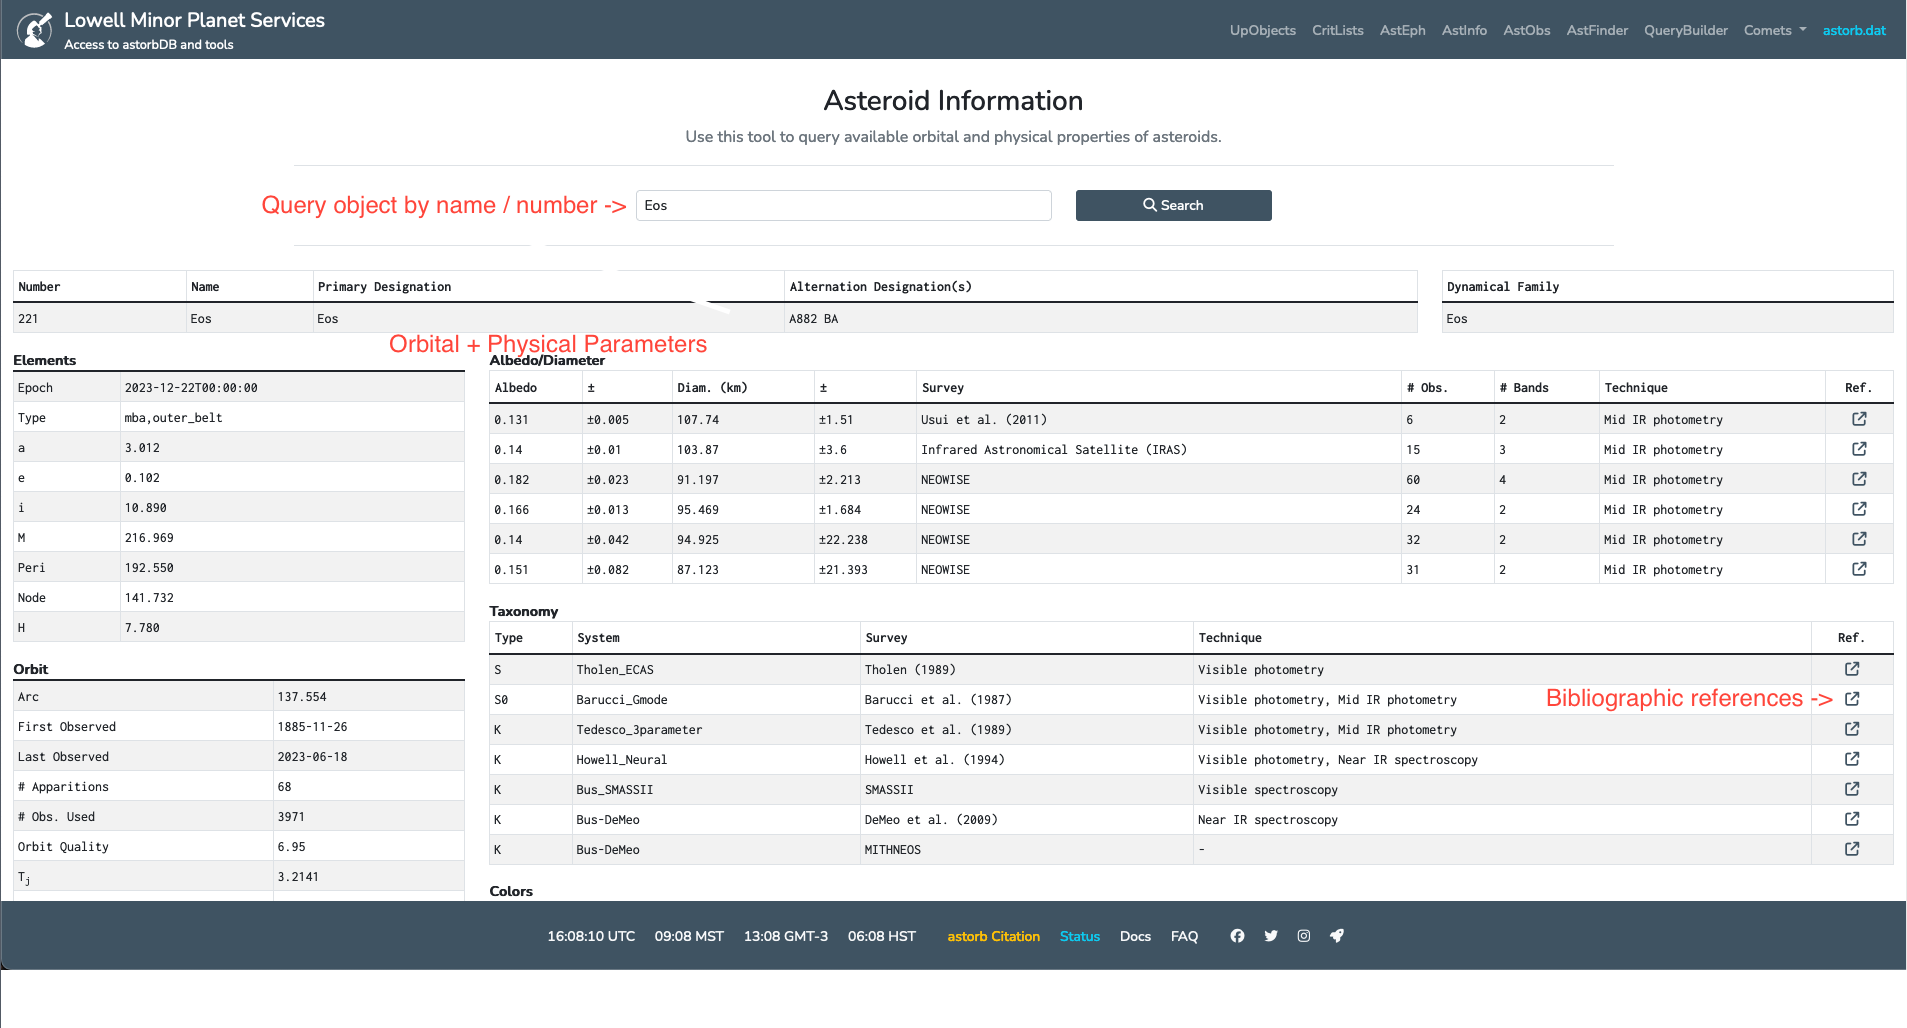
\includegraphics[width=0.9\textwidth]{gfx/demo_lowell.png}
  \url{https://asteroid.lowell.edu/}
\end{frame}

\begin{frame}[t]{Demo}
  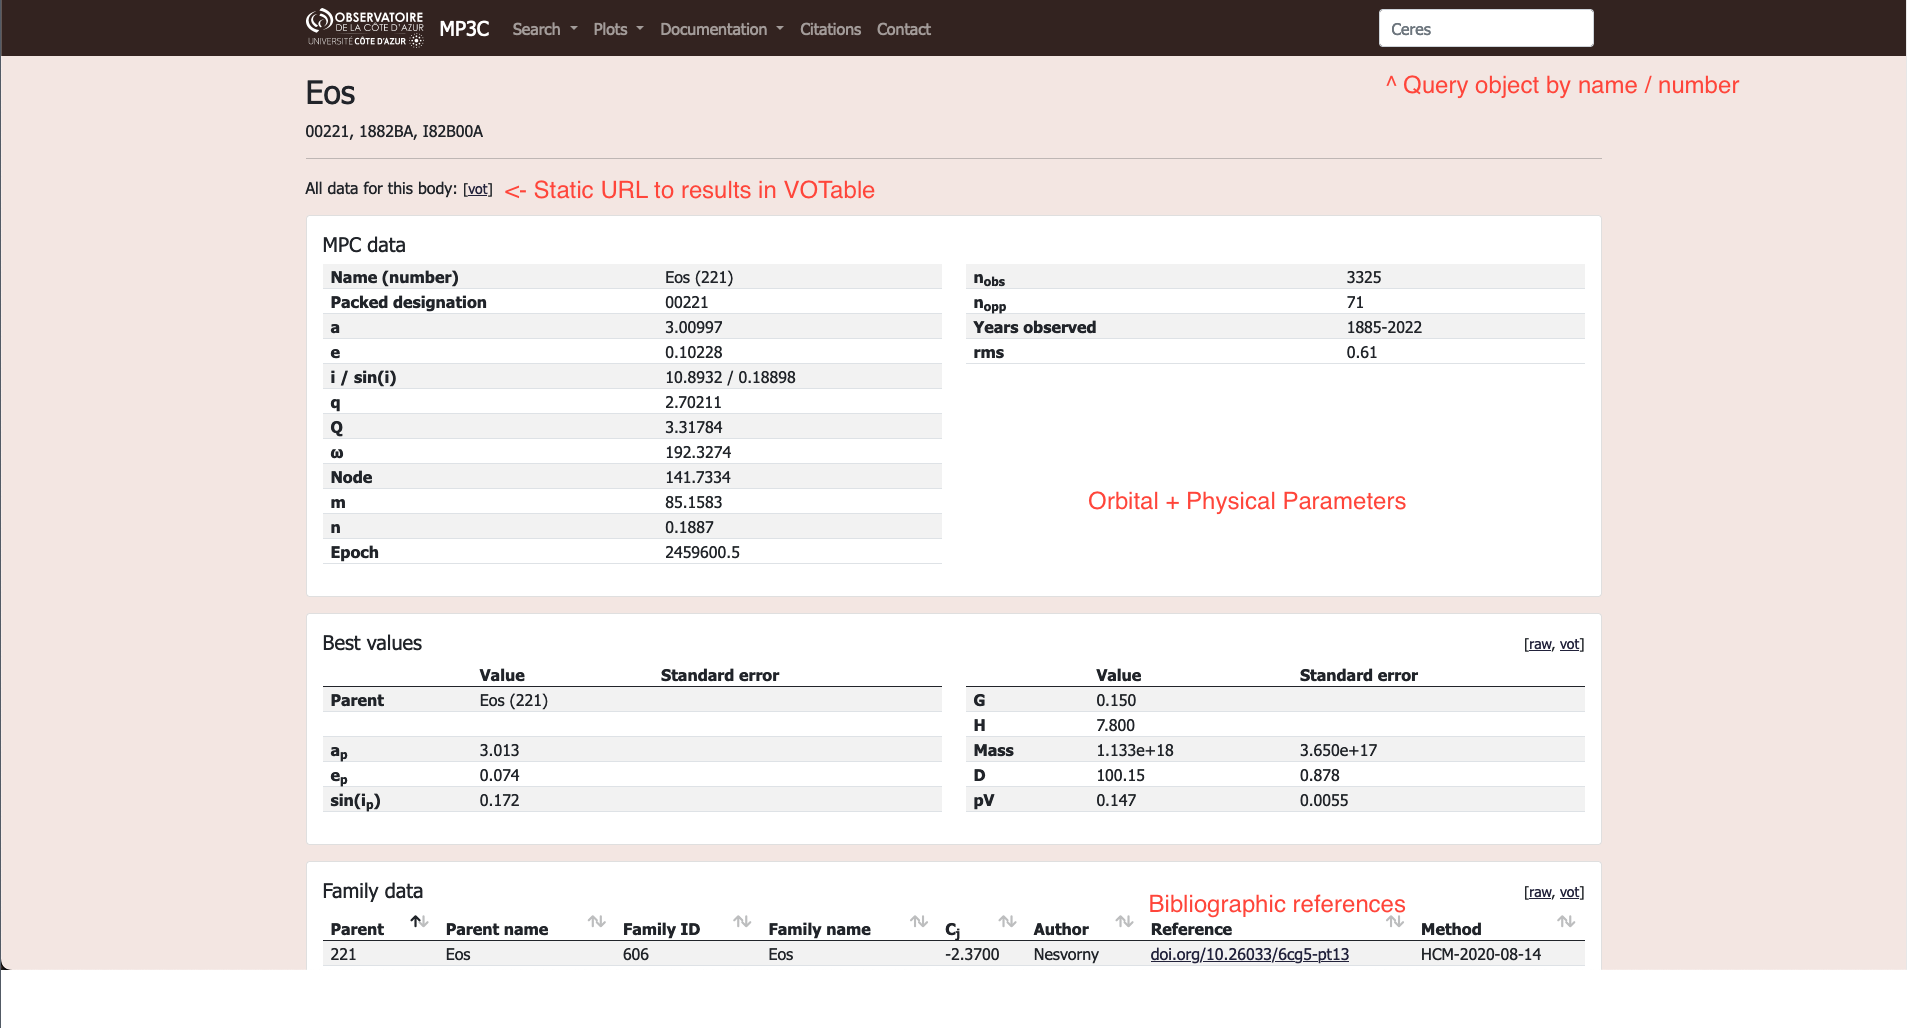
\includegraphics[width=0.9\textwidth]{gfx/demo_mp3c.png}
  \url{https://mp3c.oca.eu/}
\end{frame}

\begin{frame}[t]{Demo}
  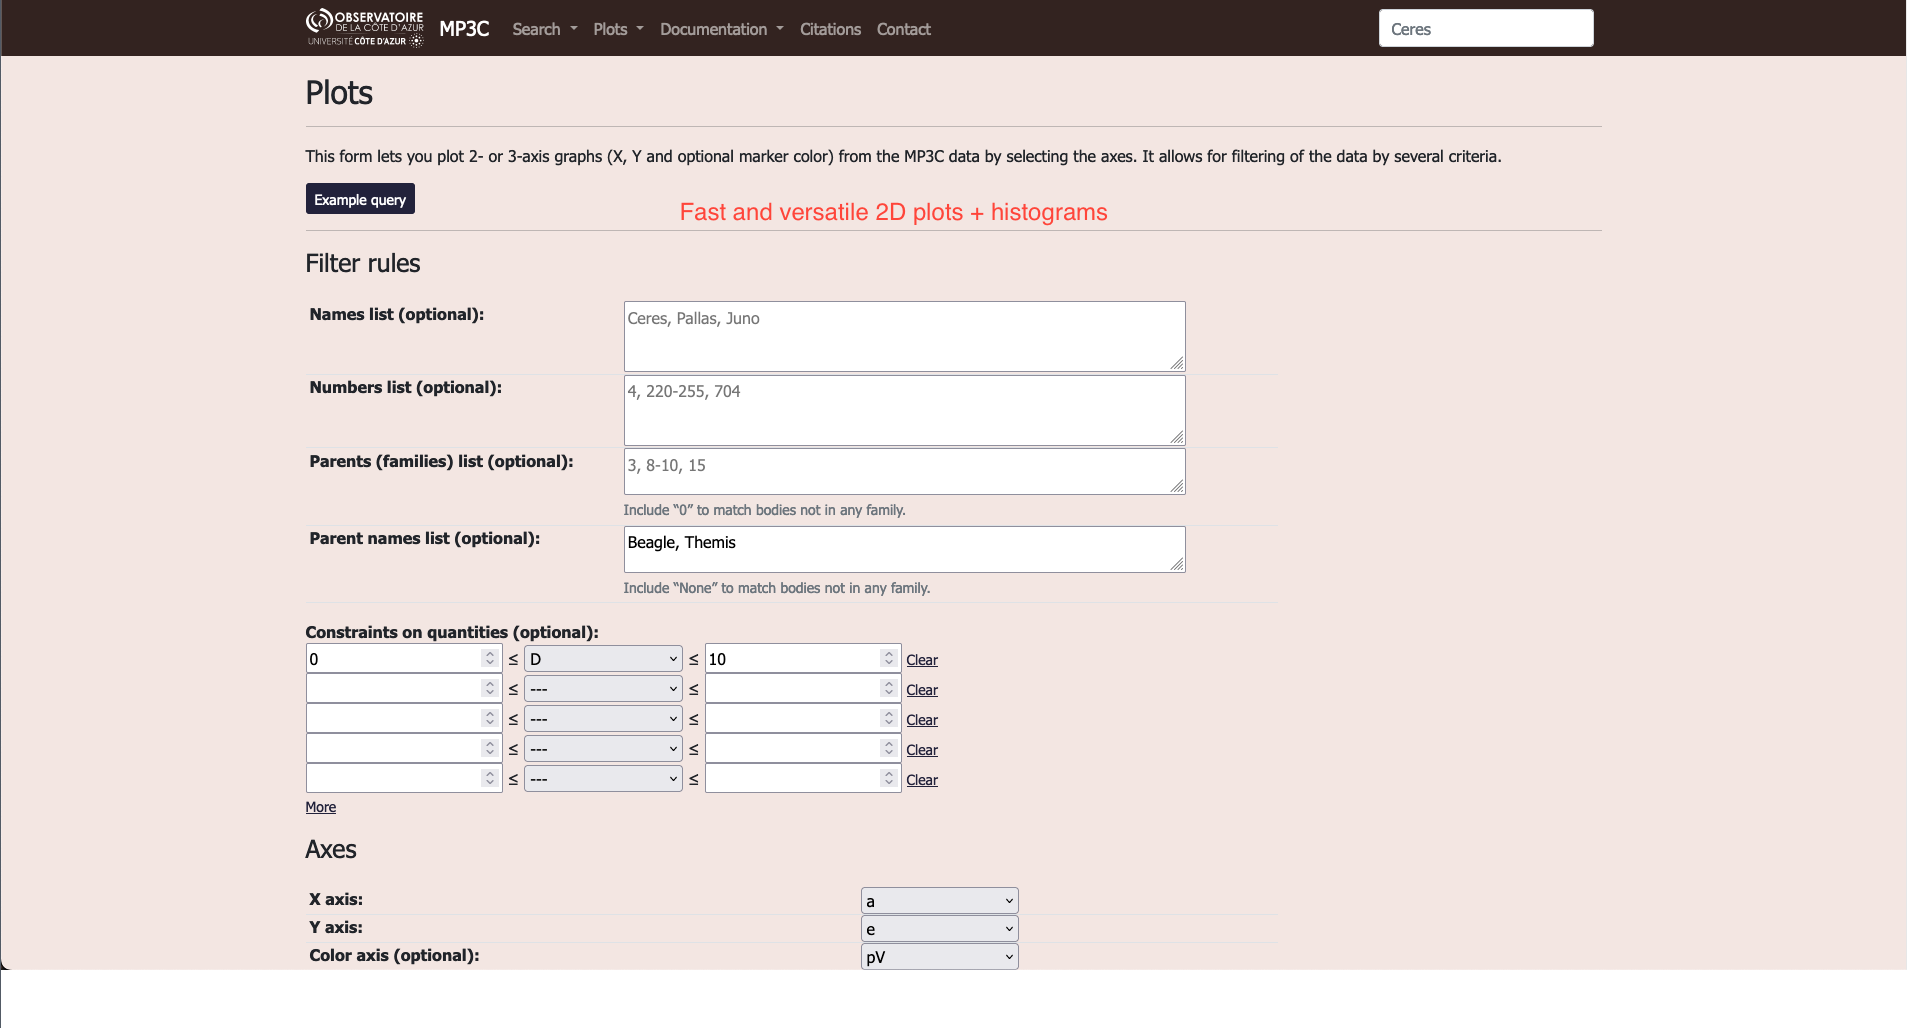
\includegraphics[width=0.9\textwidth]{gfx/demo_mp3c_2.png}
  \url{https://mp3c.oca.eu/xyc-plot/}
\end{frame}

\begin{frame}[t]{Demo}
  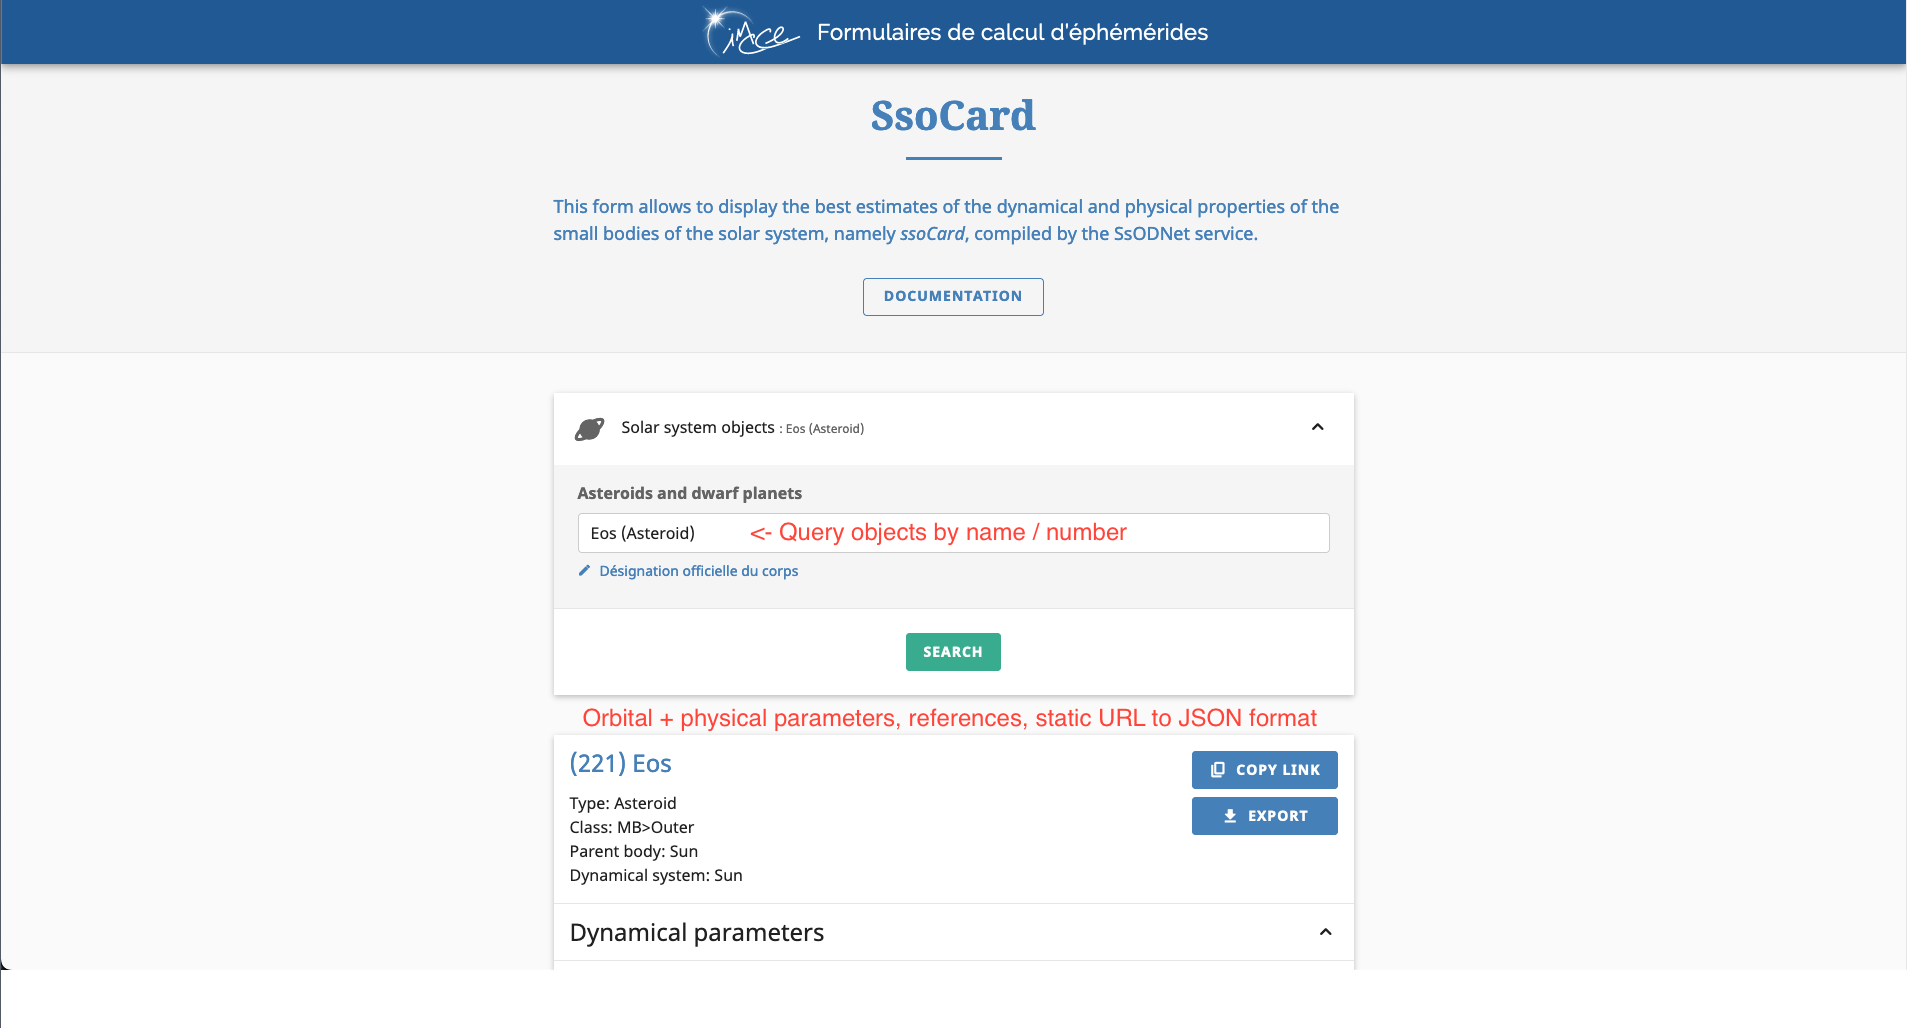
\includegraphics[width=0.9\textwidth]{gfx/demo_ssocard.png}
  \url{https://ssp.imcce.fr/forms/ssocard}
\end{frame}

\begin{frame}[t]{The N-Body Problem}

\begin{columns}[T]

      \begin{column}{.3\textwidth}
        \vspace{0.5em}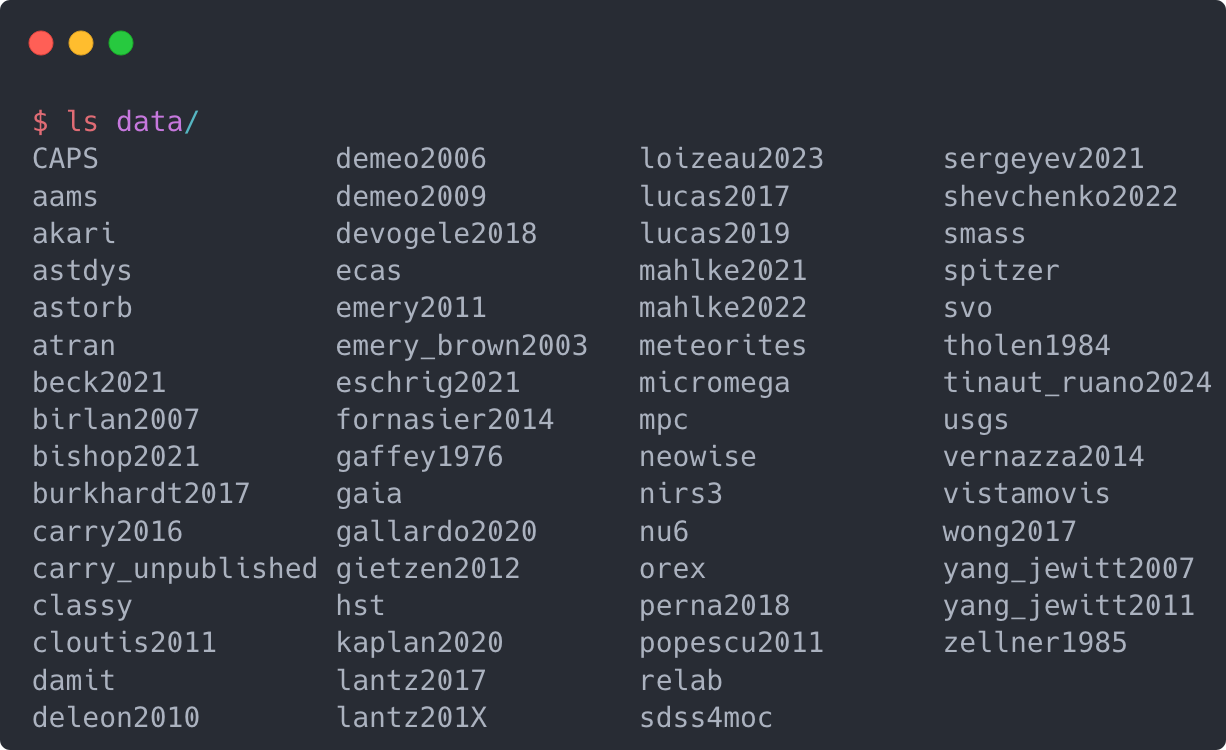
\includegraphics[width=.8\textwidth]{data_dir}\\
        \vspace{0.5em}
\includegraphics[width=.8\textwidth]{logo_astorb}\\
        \vspace{0.5em}
\includegraphics[width=.8\textwidth]{logo_mp3c}\\
        \vspace{0.5em}
\includegraphics[width=.8\textwidth]{logo_ssodnet}\\
      \end{column}


    \begin{column}{.7\textwidth}
      \begin{overlayarea}{\textwidth}{\textheight}
        \begin{onlyenv}<1>
          \vspace{1em}
          \begin{itemize}[<.->]
            \item \emph{\bf Databases}
              \begin{itemize}[<.->]
                \item[$\circ$] Different access protocols: (API), python package, TAP
                \item[$\circ$] Different degrees of simplification
                \item[$\circ$] Bibliography management
                \item[$\circ$] Python packages: API call versus object-oriented programming
                \item[$\circ$] Simplify your day-to-day with good code and databases
              \end{itemize}
          \end{itemize}
        \end{onlyenv}
      \end{overlayarea}
    \end{column}
  \end{columns}

\end{frame}

\begin{frame}[t]{Tutorial}
  [20min] Tutorial notebook on data access
\end{frame}
%%%%%%%----  END  ----  ----%%%%%%
